%-------------------------
% CV in Latex
% Auteur : Michael Lohier
% License : MIT
%------------------------

\documentclass[letterpaper,11pt]{article}

\usepackage{bold-extra}
\usepackage{latexsym}
\usepackage[empty]{fullpage}
\usepackage{titlesec}
\usepackage{marvosym}
\usepackage[usenames,dvipsnames]{color}
\usepackage{verbatim}
\usepackage{enumitem}
\usepackage[hidelinks]{hyperref}
\usepackage{fancyhdr}
\usepackage{graphicx}
\usepackage[english]{babel}
\usepackage{tabularx}
\usepackage{hyphenat}
\usepackage{fontawesome}
\usepackage{tikz}
\usepackage{graphicx}
\usepackage{xcolor}
\input{glyphtounicode}


%---------- FONT OPTIONS ----------
% sans-serif
% \usepackage[sfdefault]{FiraSans}
% \usepackage[sfdefault]{roboto}
% \usepackage[sfdefault]{noto-sans}
% \usepackage[default]{sourcesanspro}

% serif
% \usepackage{CormorantGaramond}
% \usepackage{charter}


\pagestyle{fancy}
\fancyhf{} % clear all header and footer fields
\fancyfoot{}
\renewcommand{\headrulewidth}{0pt}
\renewcommand{\footrulewidth}{0pt}

% Adjust margins
\addtolength{\oddsidemargin}{-0.5in}
\addtolength{\evensidemargin}{-0.5in}
\addtolength{\textwidth}{1in}
\addtolength{\topmargin}{-.5in}
\addtolength{\textheight}{1.0in}

\urlstyle{same}

\raggedbottom
\raggedright
\setlength{\footskip}{4.5pt}
\setlength{\tabcolsep}{0in}

% Sections formatting
\titleformat{\section}{
  \vspace{-4pt}\scshape\raggedright\large
}{}{0em}{}[\color{black}\titlerule \vspace{-5pt}]

% Ensure that generate pdf is machine readable/ATS parsable
\pdfgentounicode=1

%-------------------------
% Custom commands

\newcommand{\resumeItem}[1]{
  \item\small{
    {#1 \vspace{-2pt}}
  }
}


\newcommand{\resumeSubheading}[4]{
  \vspace{-2pt}\item
    \begin{tabular*}{0.97\textwidth}[t]{l@{\extracolsep{\fill}}r}
      \textbf{#1} & #2 \\
      \textit{\small#3} & \textit{\small #4} \\
    \end{tabular*}\vspace{-7pt}
}


\newcommand{\resumeSubSubheading}[2]{
    \vspace{-2pt}\item
    \begin{tabular*}{0.97\textwidth}{l@{\extracolsep{\fill}}r}
      \textit{\small#1} & \textit{\small #2} \\
    \end{tabular*}\vspace{-7pt}
}


\newcommand{\resumeEducationHeading}[4]{
  \vspace{-2pt}\item
    \begin{tabular*}{0.97\textwidth}[t]{l@{\extracolsep{\fill}}r}
      \textbf{#1} & #2 \\
      \textit{\small#3} & \textit{\small #4} \\
    \end{tabular*}\vspace{-5pt}
}


\newcommand{\resumeProjectHeading}[2]{
    \vspace{-2pt}\item
    \begin{tabular*}{0.97\textwidth}{l@{\extracolsep{\fill}}r}
      \small#1 & #2 \\
    \end{tabular*}\vspace{-7pt}
}


\newcommand{\resumeOrganizationHeading}[4]{
  \vspace{-2pt}\item
    \begin{tabular*}{0.97\textwidth}[t]{l@{\extracolsep{\fill}}r}
      \textbf{#1} & \textit{\small #2} \\
      \textit{\small#3}
    \end{tabular*}\vspace{-7pt}
}

\newcommand{\resumeSubItem}[1]{\resumeItem{#1}\vspace{-4pt}}

\renewcommand\labelitemii{$\vcenter{\hbox{\tiny$\bullet$}}$}

\newcommand{\resumeSubHeadingListStart}{\begin{itemize}[leftmargin=0.15in, label={}]}
\newcommand{\resumeSubHeadingListEnd}{\end{itemize}}
\newcommand{\resumeItemListStart}{\begin{itemize}}
\newcommand{\resumeItemListEnd}{\end{itemize}\vspace{-5pt}}

%-------------------------------------------
%%%%%%  CV COMMENCE ICI  %%%%%%%%%%%%%%%%%%%%%%%%%%%%


\begin{document}

%---------- PHOTO ----------

\begin{tikzpicture}[remember picture,overlay]
  \node[
    anchor=north west, inner sep=-9pt, draw=gray, line width=1.2pt, circle
  ] at ([xshift=1cm, yshift=-1.5cm]current page.north west)
  {
    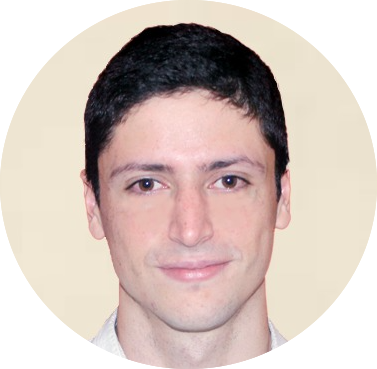
\includegraphics[width=2.5cm, height=2.5cm, keepaspectratio]{profile_cv_zoomed.png}
  };
\end{tikzpicture}

%---------- TITRE ----------

\begin{center}
    \textbf{\Huge \scshape Michael Lohier} \\ \vspace{5pt}
    {\LARGE \scshape Développeur Python} \\ \vspace{3pt}
    \small
    \faMobile \hspace{.5pt} \href{
      tel:33771827106
    }{07 71 82 71 06}
    $|$
    \faAt \hspace{.5pt} \href{
      mailto:lohiermichael@gmail.com
    }{lohiermichael@gmail.com}
    $|$
    \faLinkedinSquare \hspace{.5pt} \href{
      https://www.linkedin.com/in/lohiermichael/?locale=fr
    }{LinkedIn}
    $|$
    \faGithub \hspace{.5pt} \href{https://github.com/lohiermichael}{GitHub}
    $|$
    \faMapMarker \hspace{.5pt} \href{
      https://www.google.com/maps/place/Paris/@48.8588255,2.2646353,12z/data=!3m1!4b1!4m6!3m5!1s0x47e66e1f06e2b70f:0x40b82c3688c9460!8m2!3d48.856614!4d2.3522219!16zL20vMDVxdGo?entry=ttu
    }{Paris, France}

    \raggedright
    \vspace{10pt}
    Ayant plus de 3 ans d'expérience dans le développement Python, je suis à
    la recherche d'un poste de développeur backend. Mon expertise inclut la
    conception d'API, et l'intégration de systèmes. En autonomie ou en équipe,
    j'ai l'habitude de travailler par itération jusqu'à atteindre mes objectifs
    en suivant la méthodologie Agile.

\end{center}


%----------- DESCRIPTION -----------



%----------- EXPÉRIENCES PROFESSIONNELLES -----------

\section{Expériences professionnelles}
  \vspace{3pt}
  \resumeSubHeadingListStart

    \resumeSubheading
      {6WIND}{Paris, France}
      {Développeur Python (3 années)}
      {Mai 2021 \textbf{--} Mai 2024, CDI}

        \resumeItemListStart
            \resumeItem{
              Développement d'une API Python pour l'export de métriques via
              Telegraf vers de multiples outils de monitoring (Apache Kafka,
              Elasticsearch, Prometheus, CloudWatch...)
            }
            \resumeItem{
              Restructuration d'une API backend Python pour une CLI de
              configuration de protocoles de télécommunication.
            }
            \resumeItem{
              Mise en avant de la qualité et perfomance des produits de
              l'entreprise par la conception de dashboards Grafana.
            }
        \resumeItemListEnd

    \resumeSubheading
      {Appygas}{Berlin, Allemagne}
      {Développeur full stack (6 mois)}
      {Octobre 2020 \textbf{--} Mars 2021, CDD}

        \resumeItemListStart
            \resumeItem{
              Développement d'une application Angular deployée sur Google Cloud
              de tarification du gaz européen.
            }
            \resumeItem{
              Évolution d'une application Python/Angular en charge du
              moniotoring de crawlers web.
            }
            % \resumeItem{
            %   Collaboration avec une equipe IT remote pour mener un projet
            %   à terme en suivant la methode Agile et les Scrums
            % }
        \resumeItemListEnd

    \resumeSubheading
      {CogniteAS}{Oslo, Norvège}
      {Data scientist (6 mois)}
      {Mars 2019 \textbf{--} Septembre 2019, Stage }

        \resumeItemListStart
            \resumeItem{
              Conception d'une pipeline ETL automatisée avec Azure Databricks
              (Pyspark) réduisant les coûts de maintenance d'un client clé par
              3.
            }
            \resumeItem{
              Elaboration de tests de simulation pour une application de
              détection de pannes sur platforme gazière.
            }
            \resumeItem{
              Conception de prototypes de dashboards PowerBI en réponse à
              un appel d'offre.
            }
        \resumeItemListEnd

  \resumeSubHeadingListEnd


%----------- ÉDUCATION -----------

\section{Éducation}
  \vspace{3pt}
  \resumeSubHeadingListStart

    \resumeEducationHeading
      {IMT Mines Albi}
      {Albi, France}
      {Master généraliste \textbf{--} Spécialité: Gestion des systèmes d'information}
      {Septembre 2016 \textbf{--} Juin 2019}

    \resumeEducationHeading
      {Lycée Charlemagne}
      {Paris, France}
      {Classes Préparatoires CPGE \textbf{--} Filière: MPSI/MP, spécialité: informatique}
      {Septembre 2013 \textbf{--} Juin 2016}
  \resumeSubHeadingListEnd

%----------- COMPÉTENCES -----------


\section{Compétences}
  \vspace{2pt}
  \resumeSubHeadingListStart
    \small{\item{
        \textbf{Languages de programmation:}{
          Python 3.6+, JavaScript (ES6), TypeScript, Bash
        } \\ \vspace{3pt}
        \textbf{Développement Python:}{
          Django, Django REST Framework, Flask, FastAPI, Unittest, Pandas
        } \\ \vspace{3pt}
        \textbf{Développement JavaScript:}{
          Node.js, Express.js,  Angular, React, HTML 5, CSS 3
        } \\ \vspace{3pt}
        \textbf{Développement Cloud \& DevOps:}{
          Git, Jenkins, GitHub, Docker, GCP, AWS
        } \\ \vspace{3pt}
        \textbf{Ingénierie data:}{
          InfluxDB, Elasticsearch, Apache Kafka, Prometheus, Graphite, Grafana,
          Microsoft PowerBI
        } \\ \vspace{3pt}
        \textbf{Langues:}{
          Français (langue natale), Anglais (niveau professionnel)
        } \\ \vspace{3pt}
        \textbf{Intérêts:}{
          Jeu d'échecs, Voyages
        } \\ \vspace{3pt}
    }}
  \resumeSubHeadingListEnd


%----------- PROJETS -----------

\section{Projets}
    \vspace{3pt}
    \resumeSubHeadingListStart

      % \resumeProjectHeading
      %   {
      %     \textbf{
      %       Compétition de trading de crypto-monnaies (Golang, Solidity, AWS,
      %       Python, GraphQL)
      %     }
      %   }{}
      %     \resumeItemListStart
      %       \resumeItem{
      %         Conception d'un robot de trading en Golang avec un groupe de 7
      %         personnes.
      %       }
      %       \resumeItem{
      %         Implémentation d'une strategie d'achat scalable sur differentes
      %         Blockchains.
      %       }
            % \resumeItem{
            %   Étude du marché par analyse de données en Python et exploration de
            %   stratégies de revente.
            % }
          % \resumeItemListEnd

      \resumeProjectHeading
        {
          \textbf{
            Site web professionnel de photographie (JavaScript, Node, Express,
            HTML, CSS)
          } $|$ \emph{
            \href{
              https://github.com/lohiermichael/photography-portfolio-site
            }{\color{blue}GitHub}
          } $|$ \emph{
            \href{
              https://laurentxdubois.com
            }{\color{blue}Website}
          }
        }{}
          \resumeItemListStart
            \resumeItem{
              Re-design et développement d'un site responsif de photographie
              professionnel.
            }
            \resumeItem{
              Utilisation de Google PageSpeed Insights et d'autres outils
              d'optimisation pour monitorer et améliorer les performances du
              site Web.
            }
          \resumeItemListEnd

      \resumeProjectHeading
        {
          \textbf{
            Flappy Bird AI (Python)
          } $|$ \emph{
            \href{
              https://github.com/lohiermichael/flappy-bird-ai
            }{\color{blue}GitHub}
          }
        }{}
          \resumeItemListStart
            \resumeItem{
              Reconception du jeu Flappy Bird en intégrant de l'intelligence
              artificielle.
            }
            \resumeItem{
              Ajout d'une fonctionalité permettant à l'utilisateur d'entraîner
              son propre réseau de neurones avec un algorithme génétique afin
              d'obtenir un "flappy bird"-robot qu'il peut affronter.
            }
          \resumeItemListEnd

    \resumeSubHeadingListEnd


%----------- HOBBIES -----------

% \section{Hobbies}
%   \resumeSubHeadingListStart
%     \small{\item{Chess, Investment, Backpacking}}
%   \resumeSubHeadingListEnd

\end{document}
